\definecolor{wwwwww}{rgb}{0.4,0.4,0.4}
\definecolor{tttttt}{rgb}{0.2,0.2,0.2}

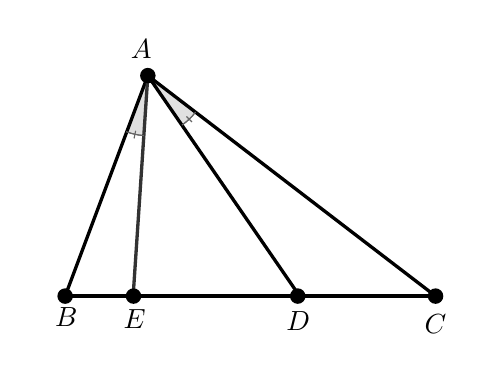
\begin{tikzpicture}[scale = 0.7]
    \clip(-7.07,1.12) rectangle (1.06,7);
    \draw [shift={(-4.89,6.13)},color=wwwwww,fill=wwwwww,fill opacity=0.2] (0,0) -- (-111.18:1.09) arc (-111.18:-93.82:1.09) -- cycle;
    \draw [shift={(-4.89,6.13)},color=wwwwww,fill=wwwwww,fill opacity=0.2] (0,0) -- (-55.44:1.09) arc (-55.44:-37.38:1.09) -- cycle;
    \draw [line width=1.2pt] (-4.89,6.13)-- (-6.39,2.13);
    \draw [line width=1.2pt] (-6.39,2.13)-- (0.33,2.13);
    \draw [line width=1.2pt] (0.33,2.13)-- (-4.89,6.13);
    \draw [line width=1.2pt,color=tttttt] (-4.89,6.13)-- (-5.15,2.23);
    \draw [line width=1.2pt] (-4.89,6.13)-- (-2.17,2.18);
    \draw [shift={(-4.89,6.13)},color=wwwwww] (-111.18:1.09) arc (-111.18:-93.82:1.09);
    \draw[color=wwwwww] (-5.11,5.13) -- (-5.14,4.99);
    \draw [shift={(-4.89,6.13)},color=wwwwww] (-55.44:1.09) arc (-55.44:-37.38:1.09);
    \draw[color=wwwwww] (-4.19,5.39) -- (-4.09,5.29);
    \begin{scriptsize}
        \normalsize
        \fill [color=black] (-4.89,6.13) circle (4pt);
        \draw[color=black] (-5.01,6.61) node {$A$};
        \fill [color=black] (-6.39,2.13) circle (4.0pt);
        \draw[color=black] (-6.37,1.75) node {$B$};
        \fill [color=black] (0.33,2.13) circle (4.0pt);
        \draw[color=black] (0.33,1.63) node {$C$};
        \fill [color=black] (-5.15,2.13) circle (4.0pt);
        \draw[color=black] (-5.13,1.72) node {$E$};
        \fill [color=black] (-2.17,2.13) circle (4.0pt);
        \draw[color=black] (-2.16,1.67) node {$D$};
    \end{scriptsize}
\end{tikzpicture}